%----------------------------------------------------------------------
\begin{frame}[c]{Where are we? The big picture}

\begin{itemize}
\item Algorithm Selection
  \begin{itemize}
    \item Portfolios
    \item Algorithm selection (for runtime)
  \end{itemize}
  \item Design decisions:\\ Local Search + Evo. Algorithms + Machine Learning 
  \item Empirical evaluation
  \item AAD for ML
  \begin{itemize}
    \item Hyperparameter optimization and Bayesian optimization 
    \item Neural architecture search (lecture given by Prof. Hutter)
  \end{itemize}
  \item Algorithm configuration 
  \begin{itemize}
    \item Basics 
    \item State of the art 
    \item Best practices 
  \end{itemize}
  \item[$\to$] Combinations of algorithm selection and configurations
  \item Algorithm control 
  \item Algorithm analysis 
  \item Project announcement and questions for exam 
\end{itemize}

\end{frame}
%----------------------------------------------------------------------
%----------------------------------------------------------------------
\begin{frame}[c]{Overview}

\centering
\scalebox{0.8}{
\tikzstyle{myarrow}=[->, ultra thick]
\begin{tikzpicture}[transform shape,line width=0.2pt]
\tikzstyle{level 1 concept}+=[sibling angle=120, level distance=125]
\path[mindmap,concept color=black!100,text=white]
    node[concept] {ML4AAD}
    [clockwise from=30]
    child[concept color=green!50!black] { node[concept] (sel) {Algorithm\\ Selection}}  
    child[concept color=orange!60!black] {node[concept] (sch) {Algorithm\\ Schedule}}
    child[concept color=red!60!black] { node[concept] (con) {Algorithm\\ Configuration}};

\end{tikzpicture}
}

\end{frame}
%----------------------------------------------------------------------
%----------------------------------------------------------------------
\begin{frame}[c]{Learning Goals}

After this lecture, you will be able to \ldots

\begin{itemize}
  \item create complementary portfolios of configurations
  \begin{itemize}
    \item Hydra
    \item ISAC
  \end{itemize}
  \item combine portfolio construction and algorithm selection
  \item build a robust algorithm selector
\end{itemize}


\end{frame}
%----------------------------------------------------------------------
%----------------------------------------------------------------------
\begin{frame}[c]{Reminder: Algorithm Configuration}

\includegraphics[width=0.9\textwidth]{images/ac_comic}

\pause

\bigskip
$\leadsto$ implicit assumption:\\ There is a configuration $\conf$ that performs well on all $\inst \in \insts$

\end{frame}
%----------------------------------------------------------------------
%----------------------------------------------------------------------
\begin{frame}[c]{Algorithm Configuration on Heterogeneous Instances}

\begin{block}{Known Problem}
Algorithm Configuration performs only well on homogeneous instance sets
\end{block}

\pause
\bigskip

\begin{block}{Open Question}
How to determine whether an instance set is heterogeneous or homogeneous?
\end{block}  

\pause
\bigskip

\begin{block}{Known Solution to the Problem}
\begin{enumerate}
  \item Use Algorithm Configuration to determine a set of complementary configurations
  \item Apply Algorithm Selection to perform well on heterogeneous instance sets
\end{enumerate}
\end{block}

\end{frame}
%----------------------------------------------------------------------
%----------------------------------------------------------------------
\begin{frame}[c]{PIAC: Per-Instance Algorithm Configuration}

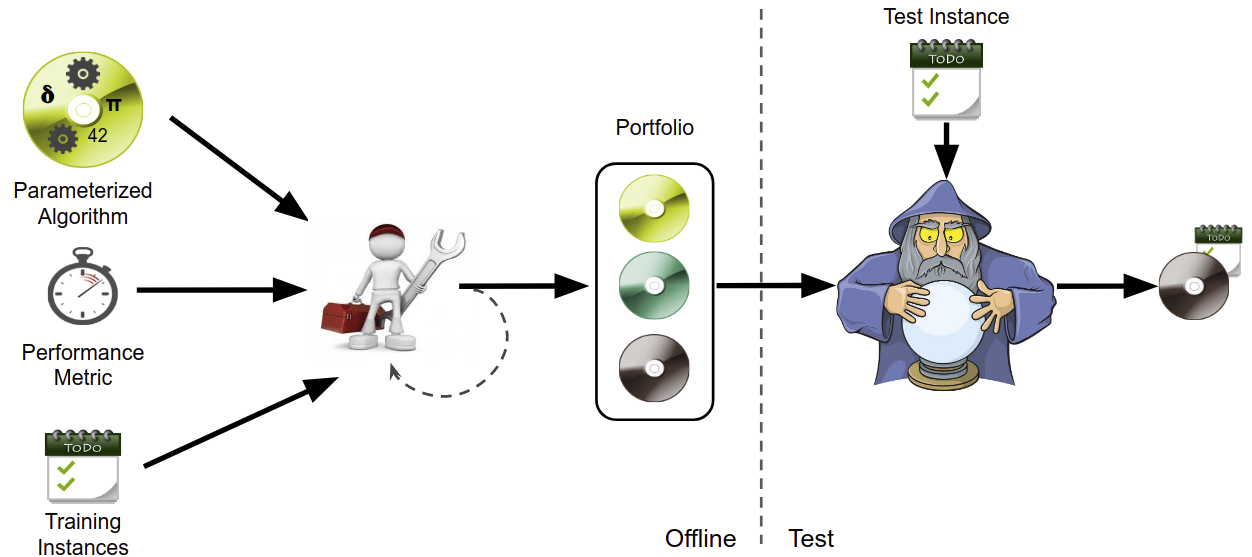
\includegraphics[width=1.\textwidth]{images/piac_full_comic}

\pause
\bigskip

\begin{itemize}
  \item You can use whichever kind of algorithm selection (wizard) you want
  \item \alert{Challenge:} Building a portfolio
  \item \alert{Use case:} Instances are heterogeneous
\end{itemize}

\end{frame}
%----------------------------------------------------------------------
%----------------------------------------------------------------------
\begin{frame}[c]{Weak Homogeneity}

\begin{block}{Weak Homogeneity}
An instance set $\insts$ is weakly homogeneous\\ if
the best configuration on each instance is the same.

\pause
\medskip
$\leadsto$ we cannot measure (weak) homogeneity\\
because we cannot guarantee that we found the best configuration.
\end{block}

\pause


\begin{block}{Approximation via \cshc{} Criterion \litw{Y. Malitsky et al. 2013}}
\begin{equation}
h(\insts) = \underbrace{\min_{\conf \in \pcs} \sum_{\inst \in \insts} c(\algo, \inst)}_{\text{single best}} - \underbrace{\sum_{\inst \in \insts} \min_{\conf \in \pcs} c(\algo, \inst)}_{oracle} \nonumber
\end{equation}

\begin{itemize}
  \item Approximate $\conf \in \pcs$ by using algorithm configuration
  \item If $h(\insts)$ is smaller, the set is more homogeneous.
\end{itemize}

\end{block}

\end{frame}
%----------------------------------------------------------------------
%----------------------------------------------------------------------
\begin{frame}[c]{Toy Examples}

\begin{columns}

\column{0.40\textwidth}
\begin{center}
\begin{tabular}{l|ccc}
& $\conf_1$ & $\conf_2$ & $\conf_3$\\
\midrule
$\inst_1$ & 1 & 3 & 2 \\
$\inst_2$ & 1 & 2 & 3 \\
$\inst_3$ & 4 & 5 & 10 \\ 
\end{tabular}
\end{center}

\bigskip
\pause
$\leadsto$ Oracle performance: $2$\\
$\leadsto$ SBS performance: $2$\\
$\leadsto$ weak homogeneous 

\pause
\column{0.40\textwidth}
\begin{center}
\begin{tabular}{l|ccc}
& $\conf_1$ & $\conf_2$ & $\conf_3$\\
\midrule
$\inst_1$ & 2 & 3 & 2 \\
$\inst_2$ & 6 & 10 & 3 \\
$\inst_3$ & 4 & 5 & 10 \\ 
\end{tabular}
\end{center}

\bigskip
\pause
$\leadsto$ Oracle performance: $3$\\
$\leadsto$ SBS performance: $4$ \\
$\leadsto$ less homogeneous

\end{columns}


\end{frame}
%----------------------------------------------------------------------
%----------------------------------------------------------------------
\begin{frame}[c]{Strong Homogeneity}

\begin{block}{Strong Homogeneity}
An instance set $\insts$ is strictly homogeneous\\
if the ranking of all configurations on each instance is the same.
\end{block}

\pause

\begin{block}{Idea \litw{Schneider and Hoos '12}}
\begin{itemize}
  \item strong homogeneity is beneficial for AC,\\ because guidance in $\pcs$ is better 
  \item easier to approximate by some sampled configurations $\pcs'$
  \item Idea: A configuration is rated by an instance\\ and these ratings should be as consistent as possible
\end{itemize}

\begin{equation}
h(\insts) = \frac{1}{|\pcs'|} \sum_{\conf \in \pcs'} \sum_{\inst \in \insts} (\mu_\conf - c (\conf, \pi))^2 \nonumber
\end{equation}

\pause
\begin{itemize}
  \item Instead of $c$, we could use ranks based on $c$ or normalize $c$ across $\pcs'$
\end{itemize}

\end{block}

\end{frame}
%----------------------------------------------------------------------
%----------------------------------------------------------------------
\begin{frame}[c]{Toy Example (cont'd)}

\begin{columns}

\column{0.40\textwidth}
\begin{center}
\begin{tabular}{l|ccc}
& $\conf_1$ & $\conf_2$ & $\conf_3$\\
\midrule
$\inst_1$ & 1 & 3 & 2 \\
$\inst_2$ & 1 & 2 & 3 \\
$\inst_3$ & 4 & 5 & 10 \\ 
\end{tabular}
\end{center}

\bigskip
\pause
$\leadsto$ strong metric: $5.40$ \\
$\leadsto$ weak metric: $0$ 

\pause
\column{0.40\textwidth}
\begin{center}
\begin{tabular}{l|ccc}
& $\conf_1$ & $\conf_2$ & $\conf_3$\\
\midrule
$\inst_1$ & 1 & 3 & 2 \\
$\inst_2$ & 1 & 2 & 3 \\
$\inst_3$ & 1 & 2 & 3 \\ 
\end{tabular}
\end{center}

\bigskip
Using ranks instead of $c$\\
$\leadsto$ less prone different instance hardness

\bigskip
\pause
$\leadsto$ strong metric: $0.14$\\
$\leadsto$ weak metric: $0$\\

\end{columns}

\end{frame}
%----------------------------------------------------------------------
%----------------------------------------------------------------------
\begin{frame}[c]{PIAC: Per-Instance Algorithm Configuration}

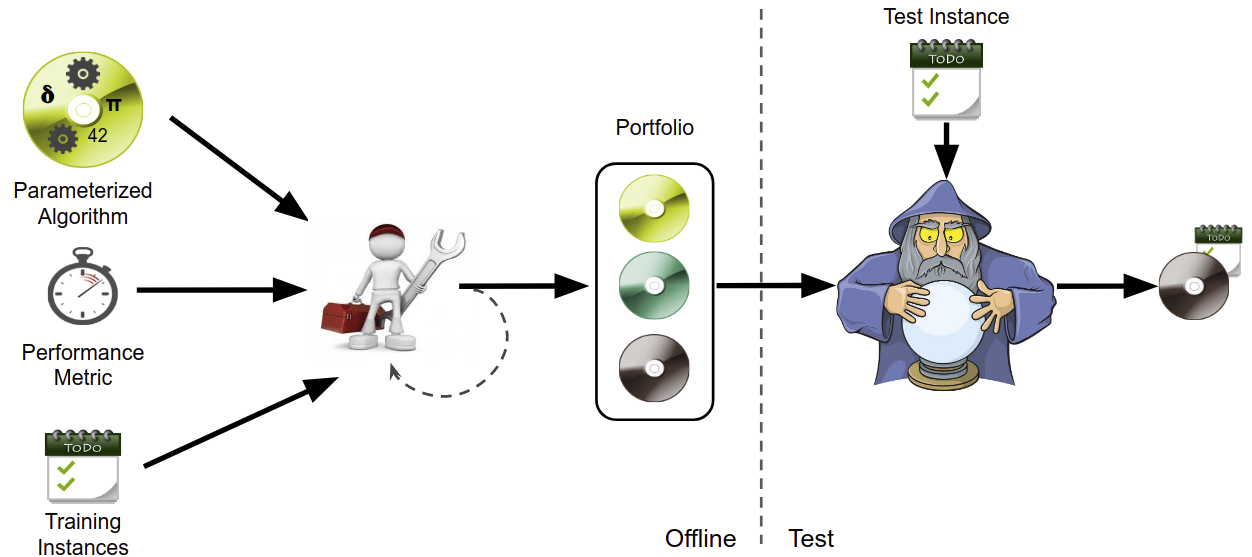
\includegraphics[width=1.\textwidth]{images/piac_full_comic}

\bigskip

\begin{itemize}
  \item You can use whichever kind of algorithm selection (wizard) you want
  \item \alert{Challenge:} Building a portfolio
  \item \alert{Use case:} Instances are heterogeneous
\end{itemize}

\end{frame}
%----------------------------------------------------------------------
%----------------------------------------------------------------------
\begin{frame}[c]{PIAC: Manual Expert Approach}

\begin{block}{Basic Assumption}
Heterogeneous instance set can be divided into homogeneous subsets
\end{block}

\pause
\bigskip

\begin{block}{Manual Expert}
\begin{itemize}
  \item An expert knows the homogeneous subsets (e.g., origin of instances)
  \item Determine a well-performing configuration on each subset\\
  		$\to$ portfolio of configurations
  \item Use Algorithm Selection to select a well-performing configuration on each instance 
\end{itemize}

\end{block}  

\medskip
\pause

How would you automate this process?\hands

\end{frame}
%----------------------------------------------------------------------
%----------------------------------------------------------------------
\begin{frame}{Instance-Specific Algorithm Configuration: \isac{}\\ \litw{S. Kadioglu et al. 2010}}


\begin{block}{Idea}
Training:
\begin{enumerate}
  \item Cluster instances into homogeneous subsets\\ (using $g$-means in the instance feature space)
  \item Apply algorithm configuration (here GGA) on each instance set
\end{enumerate}

\pause
Test:
\begin{enumerate}
  \item Determine the nearest cluster ($k$-NN with $k=1$) in feature space
  \item Apply optimized configuration of this cluster 
\end{enumerate}
\end{block}

\begin{center}
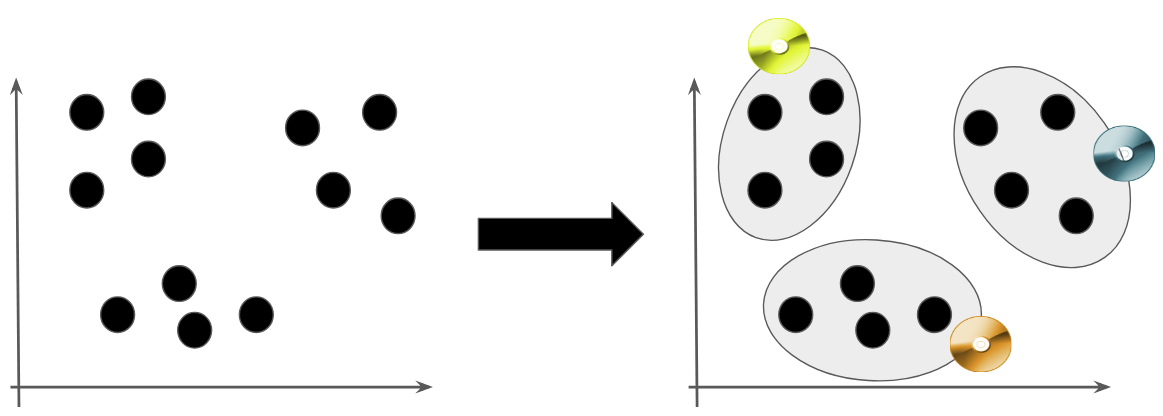
\includegraphics[width=.5\textwidth]{images/isac}
\end{center}

\end{frame}
%----------------------------------------------------------------------
%----------------------------------------------------------------------
\begin{frame}[c]{\eisac{}~\litw{Y. Malitsky et al. 2013}}

\begin{block}{Motivation}
\begin{itemize}
  \item Over time, the underlying distribution of $\insts$ changes
  \item All-encompassing training set does not exist
  \item Selector should evolve over time
\end{itemize}
\end{block}

\bigskip
\pause

\begin{block}{Idea}
\begin{itemize}
  \item Update cluster if we see instances that are not represented 
  \item Update configuration selection for a cluster if a cluster gets more instances
  \item Add and remove configurations, and update clusters
\end{itemize}
\end{block}

\end{frame}
%----------------------------------------------------------------------
%----------------------------------------------------------------------
\begin{frame}[c]{\isac{}+ \litw{Y. Malitsky et al. 2014}}

\begin{block}{Observations}
\begin{itemize}
  \item Not important to apply the configuration found on a cluster
  \item Arbitrary algorithm selection approach possible 
\end{itemize}
\end{block}

\pause
\medskip

\begin{block}{Idea}
\begin{enumerate}
  \item Cluster instances
  \item Apply algorithm configuration on each cluster
  \item Assess the performance of all configurations on each instance
  \item Use cost-sensitive hierarchical clustering (CSHC; see lecture on AS)
\end{enumerate}
\end{block}

\end{frame}
%----------------------------------------------------------------------
%----------------------------------------------------------------------
\begin{frame}[c]{\hydra~\litw{X. Lin et al. 2010}}

\begin{block}{Idea}
\begin{itemize}
  \item Iteratively add configurations to a portfolio $\portfolio$, start with $\portfolio = \emptyset$
  \item In each iteration, determine configuration that is complementary to~$\portfolio$
  \begin{itemize}
    \item[$\leadsto$] Maximize marginal contribution to $\portfolio$
  \end{itemize}
\end{itemize}

\pause

Marginal contribution of a configuration $\theta$ to a portfolio $\portfolio$:
\begin{equation}
c(\portfolio) -  c(\portfolio \cup \{\conf\})  \nonumber
\end{equation}

\end{block}

\pause

\scalebox{0.8}{
\centering

\begin{tikzpicture}[node distance=5cm, thick]
	%PreProcessing
	%\node (Algo) [data] {Algorithm $A$};
	\node (Data) [data] {Instances $\insts$};
	\node (CS) [data, right of=Data, xshift=-0.5cm] {Algorithm $\algo$ and\\ its Configuration\\ Space $\confs$};
	\node (Select) [activity, below of=Data, node distance=2.0cm] {Select $\conf \in \confs$\\ and $\inst \in \insts$};
	\node (Run) [activity, right of=Select, xshift=-0.5cm] {\only<2-3>{Assess\\ $\algo(\conf)$ on $\inst$}%
															\only<4-5>{Assess $\algo(\conf||\conf_1)$ on $\inst$}
															\only<6-6>{Assess $\algo(\conf||\conf_1||\conf_2)$ on $\inst$}};
	%\node (Return) [activity, right of=Run, text width=9em] {Return Performance\\ of $A(c)$ on $I'$}; 
	%\node (Data) [data, left of=Select] {Instances $I$};	
	\node (Result) [data, right of=Run, node distance=5.5cm] { $\portfolio = $\only<2-2>{$\{\}$}%
																\only<3-4>{$\{\conf_1\}$}%
																\only<5->{$\{\conf_1,\conf_2\}$}%
																}; 
	
	\draw[myarrow] (Data) -- ($(Select)+(-0.0,+0.8)$);
	\draw[myarrow] (CS) -- ($(Run)+(-0.0,+0.8)$);
	%\draw[myarrow] (Data) -- ($(Select)+(-2.1,+0.0)$);
	
	%\draw[thick, dashed] (Algo) -- (CS);
	\only<3-3>{\draw[myarrow] ($(Run.east)+(0.25,.1)$) to [bend angle=60, bend left] node[above] {\footnotesize $\conf_1$} ($(Result.west)+(0.0,.1)$);}
	\only<5-5>{\draw[myarrow] ($(Run.east)+(0.25,.1)$) to [bend angle=60, bend left] node[above] {\footnotesize $\conf_2$} ($(Result.west)+(0.0,.1)$);}
	\only<2-2>{\draw[myarrow] ($(Result.west)+(0.0,-.1)$) to [bend angle=60, bend left] node[below] {\footnotesize $\{\}$} ($(Run.east)+(0.25,-.1)$);}
	\only<4-4>{\draw[myarrow] ($(Result.west)+(0.0,-.1)$) to [bend angle=60, bend left] node[below] {\footnotesize $\{\conf_1\}$} ($(Run.east)+(0.25,-.1)$);}
	\only<6-6>{\draw[myarrow] ($(Result.west)+(0.0,-.1)$) to [bend angle=60, bend left] node[below] {\footnotesize $\{\conf_1,\conf_2\}$} ($(Run.east)+(0.25,-.1)$);}
	\draw[myarrow] (Select) -- (Run);
	%\draw[myarrow] (Run) -- (Return);
	\draw[myarrow] (Run.south) |- ++(0.0,-0.8)  node[above, xshift=-2.2cm] {Return $\min\left\{c(\theta), c(\portfolio) \right\}$} -| (Select.south);
	
	\begin{pgfonlayer}{background}
    
        % Configuration Process
    	\path (Select -| Select.west)+(-0.25,0.85) node (resUL) {};
    	\path (Run.east |- Run.south)+(0.25,-1.3) node(resBR) {};
    	\path [rounded corners, draw=black!20, dashed] (resUL) rectangle (resBR);
		\path (Run.east |- Run.south)+(-1.5,-1.1) node [text=black!60] {Configuration Task};
    	
    \end{pgfonlayer}
	
\end{tikzpicture}

}

\end{frame}
%----------------------------------------------------------------------
%----------------------------------------------------------------------
% !TeX spellcheck = en_US
\begin{frame}[c]{Heterogeneous example}
	\begin{figure}
		\centering
			\begin{tikzpicture}
			%	\draw[very thin,color=gray] (-0.1,-1.1) grid (3.9,3.9);
			\draw[->] (-0.2,0) -- (4.2,0) node[right] {${\conf}$};
			\draw[->] (0,-0.2) -- (0,4.2) node[above] {$c_{\inst_i}({\conf})$};
			\draw[color=blue,domain=3:7]   plot (\x-3,{sin((\x-2) r) + 1.275})   node[right] {$\inst_0({\conf})$};
			\draw[color=orange,domain=0:4] plot (\x,{0.05*exp(\x)}) node[right] {$\inst_1({\conf})$};
			\draw[color=red,domain=-2:2] plot (\x+2,{\x*\x}) node[right] {$\inst_2({\conf})$};
			
			\only<2->{
				 \foreach \x/\xtext in {0/{\conf}_{\inst_1}^*, 2/{\conf}_{\inst_2}^*, 3.725/{\conf}_{\inst_0}^*}
					\draw[shift={(\x,0)}] (0pt,2pt) -- (0pt,-2pt) node[below] {$\xtext$};
			}
			\only<3->{
				 \foreach \y/\ytext in {.75/c_{{\conf}_{SB}}}
					\draw[shift={(0,\y)}] (2pt,0pt) -- (-2pt,0pt) node[left] {$\ytext$};
				 \foreach \x/\xtext in {2.725/{\conf}_{SB}}
					\draw[shift={(\x,0)}] (0pt,2pt) -- (0pt,-2pt) node[below] {$\xtext$};
				 \draw[densely dotted,color=gray] (0,0.75) -- (2.725,.75);
				 \draw[densely dotted,color=gray] (2.725,0) -- (2.725,.75);
			}
			\only<4->{
			%	\draw[dashed,color=gray] (0,0.1275) -- (3.725,0.1275);
				\foreach \y/\ytext in {0.1275/c_{oracle}}
				\draw[shift={(0,\y)}] (2pt,0pt) -- (-2pt,0pt) node[left] {$\ytext$};
			}
			\end{tikzpicture}
	\end{figure}
\end{frame}

\begin{frame}[c]{Hydra: Iteration 1}
		\centering
		\begin{tikzpicture}
		
			\only<1>{
				%	\draw[very thin,color=gray] (-0.1,-1.1) grid (3.9,3.9);
				\draw[->] (-0.2,0) -- (4.2,0) node[right] {${\conf}$};
				\draw[->] (0,-0.2) -- (0,4.2) node[above] {$c_{\inst_i}({\conf})$};
				\draw[color=blue,domain=3:7]   plot (\x-3,{sin((\x-2) r) + 1.275})   node[right] {$\inst_0({\conf})$};
				\draw[color=orange,domain=0:4] plot (\x,{0.05*exp(\x)}) node[right] {$\inst_1({\conf})$};
				\draw[color=red,domain=-2:2] plot (\x+2,{\x*\x}) node[right] {$\inst_2({\conf})$};
				
%				\foreach \y/\ytext in {.75/c_{{\conf}_{0}}}
%				\draw[shift={(0,\y)}] (2pt,0pt) -- (-2pt,0pt) node[left] {$\ytext$};
				\foreach \x/\xtext in {2.725/{\conf}_{0}}
				\draw[shift={(\x,0)}] (0pt,2pt) -- (0pt,-2pt) node[below] {$\xtext$};
%				\draw[densely dotted,color=gray] (0,0.75) -- (2.725,.75);
				\draw[densely dotted,color=gray] (2.725,0) -- (2.725,4);
			}
			\only<2>{
				%Update metric
				%	\draw[very thin,color=gray] (-0.1,-1.1) grid (3.9,3.9);
				\draw[->] (-0.2,0) -- (4.2,0) node[right] {${\conf}$};
				\draw[->] (0,-0.2) -- (0,4.2) node[above] {$c_{\inst_i}^{'}({\conf})$};
				
				\draw[color=orange,domain=0:2.725] plot (\x,{0.05*exp(\x)});
				\draw[color=orange,domain=2.725:4] plot (\x,.75) node[right] {$\inst_1({\conf})$};
				
				\draw[color=red,domain=-.725:.725] plot (\x+2,{\x*\x});
				\draw[color=red,domain=-2:-.725] plot (\x+2,0.525625);
				\draw[color=red,domain=.725:2] plot (\x+2,0.525625) node[right] {$\inst_2({\conf})$};
				
				\draw[color=blue,domain=5.725:7]   plot (\x-3,{sin((\x-2) r) + 1.275})   node[right] {$\inst_0({\conf})$};
				\draw[color=blue,domain=3:5.725]   plot (\x-3,.75);
				
				\foreach \y/\ytext in {.75/c^{'}_{\inst_{\left\{0, 1\right\}}}(\portfolio)}
				\draw[shift={(0,\y)}] (2pt,0pt) -- (-2pt,0pt) node[left,yshift=0.15cm] {$\ytext$};
				\foreach \y/\ytext in {0.525625/c^{'}_{\inst_{2}}(\portfolio)}
				\draw[shift={(0,\y)}] (2pt,0pt) -- (-2pt,0pt) node[left,yshift=-0.15cm] {$\ytext$};
				
				\foreach \x/\xtext in {2.725/{\conf}_{0}}
				\draw[shift={(\x,0)}] (0pt,2pt) -- (0pt,-2pt) node[below] {$\xtext$};
				
%				\draw[densely dotted,color=gray] (0,0.75) -- (2.725,.75);
				\draw[densely dotted,color=gray] (2.725,0) -- (2.725,.75);
			}
		\end{tikzpicture}

			\only<1>{Search initial well performing configuration. Add ${\conf}_{0}$ to $\portfolio$}
			\only<2>{Update metric}
\end{frame}



\begin{frame}[c]{Hydra: Iteration 2}
	\centering
	\begin{tikzpicture}
	\only<1>{
		%Update metric
		%	\draw[very thin,color=gray] (-0.1,-1.1) grid (3.9,3.9);
		\draw[->] (-0.2,0) -- (4.2,0) node[right] {${\conf}$};
		\draw[->] (0,-0.2) -- (0,4.2) node[above] {$c_{\inst_i}^{'}({\conf})$};
		
		\draw[color=orange,domain=0:2.725] plot (\x,{0.05*exp(\x)});
		\draw[color=orange,domain=2.725:4] plot (\x,.75) node[right] {$\inst_1({\conf})$};
		
		\draw[color=red,domain=-.725:.725] plot (\x+2,{\x*\x});
		\draw[color=red,domain=-2:-.725] plot (\x+2,0.525625);
		\draw[color=red,domain=.725:2] plot (\x+2,0.525625) node[right] {$\inst_2({\conf})$};
		
		\draw[color=blue,domain=5.725:7]   plot (\x-3,{sin((\x-2) r) + 1.275})   node[right] {$\inst_0({\conf})$};
		\draw[color=blue,domain=3:5.725]   plot (\x-3,.75);
		
		\foreach \y/\ytext in {.75/}
		\draw[shift={(0,\y)}] (2pt,0pt) -- (-2pt,0pt) node[left,yshift=0.15cm] {$\ytext$};
		\foreach \y/\ytext in {0.525625/}
		\draw[shift={(0,\y)}] (2pt,0pt) -- (-2pt,0pt) node[left,yshift=-0.15cm] {$\ytext$};
		
		\foreach \x/\xtext in {2.725/{\conf}_{0}, 3.725/{\conf}_{1}}
		\draw[shift={(\x,0)}] (0pt,2pt) -- (0pt,-2pt) node[below] {$\xtext$};
		
%		\draw[densely dotted,color=gray] (0,0.75) -- (2.725,.75);
		\draw[densely dotted,color=gray] (2.725,0) -- (2.725,.75);
		\draw[densely dotted,color=gray] (3.725,0) -- (3.725,4);
	}

	\only<2>{
		%Update metric
		%	\draw[very thin,color=gray] (-0.,-.) grid (3.9,3.9);
		\draw[->] (-0.2,0) -- (4.2,0) node[right] {${\conf}$};
		\draw[->] (0,-0.2) -- (0,4.2) node[above] {$c_{\inst_i}^{''}({\conf})$};
		
		\draw[color=orange,domain=0:2.725] plot (\x,{0.05*exp(\x)});
		\draw[color=orange,domain=2.725:4] plot (\x,.75) node[right] {$\inst_({\conf})$};
		
		\draw[color=red,domain=-.725:.725] plot (\x+2,{\x*\x});
		\draw[color=red,domain=-2:-.725] plot (\x+2,0.525625);
		\draw[color=red,domain=.725:2] plot (\x+2,0.525625) node[right] {$\inst_2({\conf})$};
		
		\draw[color=blue,domain=0:4]   plot (\x,.25)   node[right] {$\inst_0({\conf})$};
%		\draw[color=blue,domain=3:5.725]   plot (\x-3,.75);
		
		\foreach \y/\ytext in {.75/}
		\draw[shift={(0,\y)}] (2pt,0pt) -- (-2pt,0pt) node[left,yshift=0.cm] {$\ytext$};
		\foreach \y/\ytext in {0.525625/}
		\draw[shift={(0,\y)}] (2pt,0pt) -- (-2pt,0pt) node[left,yshift=-0.0cm] {$\ytext$};
		\foreach \y/\ytext in {0.25/}
		\draw[shift={(0,\y)}] (2pt,0pt) -- (-2pt,0pt) node[left,yshift=-0.0cm] {$\ytext$};
		
		\foreach \x/\xtext in {2.725/{\conf}_{0}, 3.725/{\conf}_{1}}
		\draw[shift={(\x,0)}] (0pt,2pt) -- (0pt,-2pt) node[below] {$\xtext$};
		
				\draw[densely dotted,color=gray] (0,0.75) -- (2.725,.75);
		\draw[densely dotted,color=gray] (2.725,0) -- (2.725,.75);
		\draw[densely dotted,color=gray] (3.725,0) -- (3.725,.25);
	}
	\end{tikzpicture}
	
		\only<1>{Search well performing configuration complementary to $\portfolio$.\\Add ${\conf}_{1}$ to $\portfolio$.}
		\only<2>{Update metric}
\end{frame}
%----------------------------------------------------------------------
%----------------------------------------------------------------------
\begin{frame}[c]{\hydra{} with several runs}

\begin{itemize}
  \item Algorithm configuration is typically randomized
  \item[$\leadsto$] Several runs of configuration in each Hydra iteration
\end{itemize}

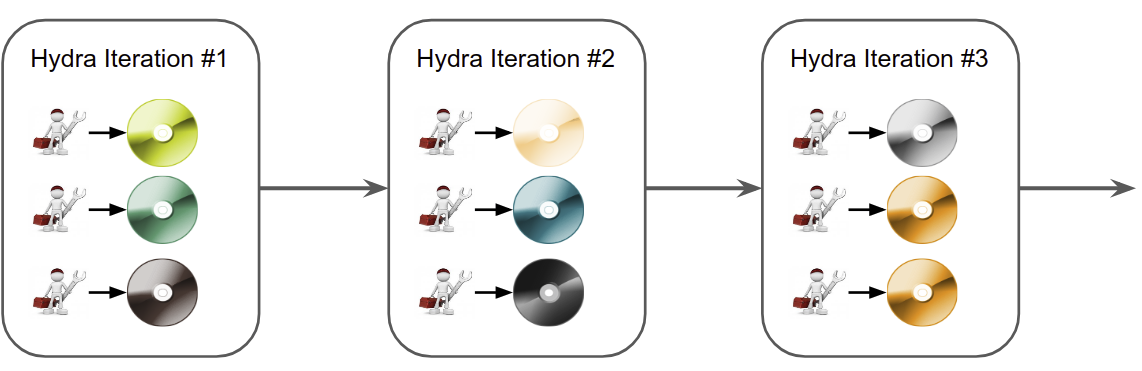
\includegraphics[width=1.0\textwidth]{images/hydra_iterations}

\pause

\medskip
$\leadsto$ How to select the configurations for the portfolio after each iteration?

\end{frame}
%----------------------------------------------------------------------
%----------------------------------------------------------------------
\begin{frame}[c]{\hydra{} Portfolio Building: One at a time~\litw{Xu et al. ‘10}}

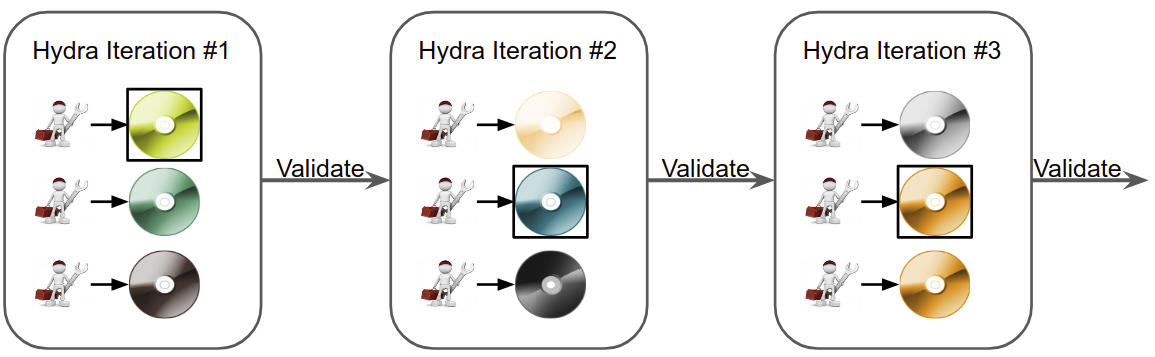
\includegraphics[width=1.0\textwidth]{images/hydra_selection1}

\end{frame}
%----------------------------------------------------------------------
%----------------------------------------------------------------------
\begin{frame}[c]{\hydra{} Portfolio Building: $k$ at a time~\litw{Xu et al. ‘11}}

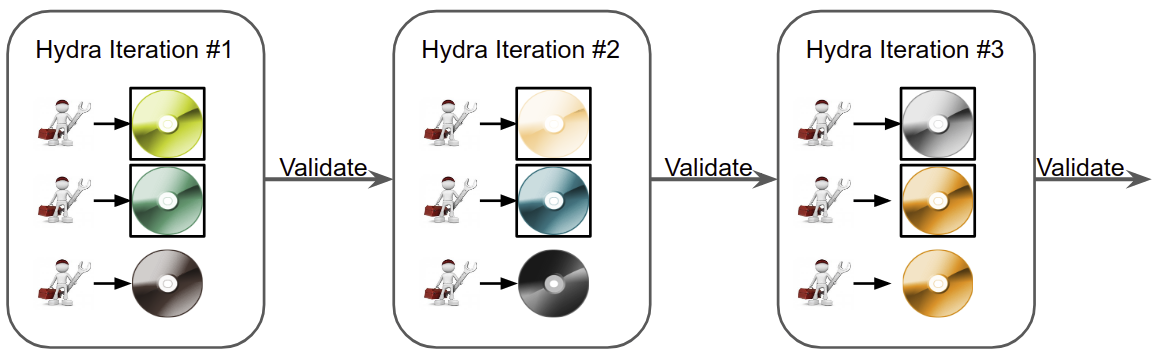
\includegraphics[width=1.0\textwidth]{images/hydra_selection2}

\end{frame}
%----------------------------------------------------------------------
%----------------------------------------------------------------------
\begin{frame}[c]{\hydra{} Portfolio Building: Round-Robin~\litw{Levesque et al. ‘16}}

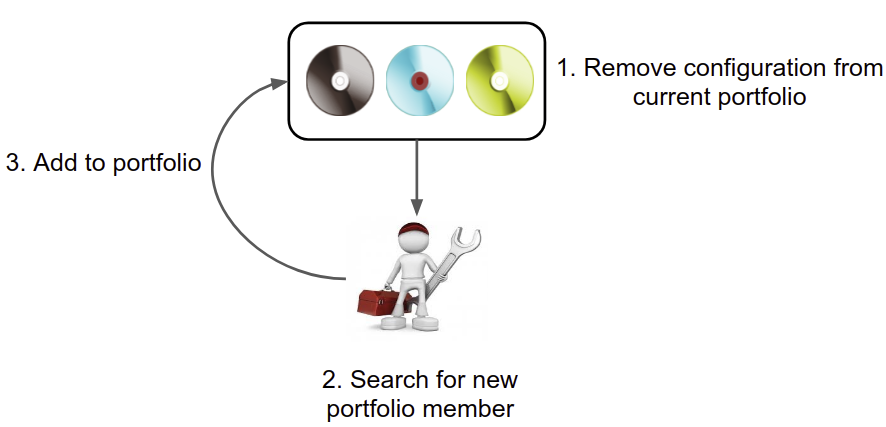
\includegraphics[width=1.0\textwidth]{images/hydra_selection3}

\end{frame}
%----------------------------------------------------------------------

%----------------------------------------------------------------------
\begin{frame}[c]{\hydra{} Portfolio Building: Hydra$^{\text{Hydra}}$}

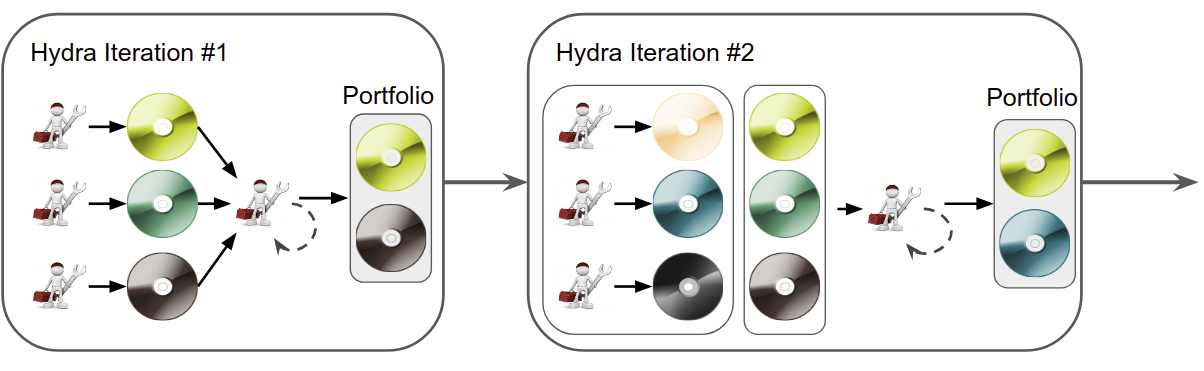
\includegraphics[width=1.0\textwidth]{images/hydra_selection4}

\bigskip
\pause
$\leadsto$ preliminary experiments indicate that Hydra$^{\text{Hydra}}$ is the best approach

\end{frame}
%----------------------------------------------------------------------
%----------------------------------------------------------------------
\begin{frame}[c]{\cedalion~\litw{J. Seipp et al 2014}}

\begin{block}{Idea}
\begin{itemize}
  \item Optimize a schedule of configurations with algorithm configuration 
\end{itemize}
\end{block}

\medskip
\pause

\begin{block}{Approach}
\begin{itemize}
  \item Iteratively add a configuration with a time slot $t$ to a schedule $\schedule \oplus \langle\conf,t\rangle$
  \pause
  \item In each iteration, only optimize on instances not solved so far
  \item The time slot is a further parameter in the configuration space
  \pause
  \item Optimize marginal contribution per time spent: 
\end{itemize}

\begin{equation}
\frac{c(\schedule) - c(\schedule \oplus \langle\conf,t\rangle)}{t} \nonumber
\end{equation}
\end{block}

\end{frame}
%----------------------------------------------------------------------
%----------------------------------------------------------------------
\begin{frame}[c]{Submodularity}

\begin{block}{Observation}
\begin{itemize}
  \item Performance metrics of \hydra{} and \cedalion{} are submodular
  \begin{itemize}
    \item Family of functions
    \item Adding an element to a set reduces the function value
    \item Diminishing returns: decrease of the value reduction over time
  \end{itemize}
\end{itemize}
\end{block}

\pause

\begin{definition}[Submodularity of $f$]
For every $X,Y \subseteq Z$ with $X \subseteq Y$ and every $x \in Z - Y$ we have that $f(X \cup \{x\}) - f(X) \geq f(Y \cup \{x\}) - f(Y)$
\end{definition}

\pause

\begin{block}{Advantage}
We can bound the error of the portfolio/schedule:\\ 
At most away from optimum by factor of $0.63$ (see \lit{Streeter \& Golovin '07})
\end{block}

\end{frame}
%----------------------------------------------------------------------
%----------------------------------------------------------------------
\begin{frame}[c]{Dynamic Instance Grouping \litw{Liu et al.'18}}

\begin{block}{Idea}
\begin{itemize}
  \item Similar to ISAC: group instances into clusters
  \item Similar to Hydra: refine clusters and configurations over several iterations 
\end{itemize}
\end{block}

\pause

\begin{block}{Main Idea}
\begin{enumerate}
  \item Group instances randomly into clusters
  \item run AC on each cluster
  \item Update clusters based on performance (estimates)
  \item Go to 2. if budget is not empty
  \item Consider all configurations ever found to create final portfolio
\end{enumerate}

\pause

\begin{itemize}
  \item increase the configuration budget in each iteration
  \begin{itemize}
    \item first clusterings will have a poor quality $\to$ small configuration time
    \item later clusterings will be better $\to$ more configuration time
  \end{itemize}
\end{itemize}

\end{block}

\end{frame}
%----------------------------------------------------------------------
%----------------------------------------------------------------------
\begin{frame}[c]{Further Combinations}

\centering
\scalebox{0.8}{
\tikzstyle{myarrow}=[->, ultra thick]
\begin{tikzpicture}[transform shape,line width=0.2pt]
\tikzstyle{level 1 concept}+=[sibling angle=120, level distance=125]
\path[mindmap,concept color=black!100,text=white]
    node[concept] {ML4AAD}
    [clockwise from=30]
    child[concept color=green!50!black] { node[concept] (sel) {Algorithm\\ Selection}}  
    child[concept color=orange!60!black] {node[concept] (sch) {Algorithm\\ Schedule}}
    child[concept color=red!60!black] { node[concept] (con) {Algorithm\\ Configuration}};
    
\path
     ($(sel.west)+(0.15,+0.65)$) edge [myarrow, bend left=20,text width=3.8cm, font=\small] node[above, yshift=.1cm] {Selection of Configurators} ($(con.east)+(-0.10,+0.55)$)
     ($(con.east)+(-0.15,+0.65)$) edge [myarrow, bend left=40,text width=4cm, font=\small] node[above] {Configuration of Selectors} ($(sel.west)+(0.15,+0.75)$)
     (sel.south) edge [myarrow, bend left=50] node[right,text width=2cm, font=\small,xshift=.05cm] {Selection of Schedules} ($(sch.east)+(0,-0.1)$)
     (sch.east) edge [myarrow, bend left=25] node[right,text width=2cm, font=\small,xshift=.05cm] {Schedules of Selectors} ($(sel.south)+(-0.05,-0.05)$)
     (sch.west) edge [myarrow, bend left=50] node[left,text width=2.4cm, font=\small, xshift=.3cm] {Schedules of Configurators} ($(con.south)+(0,-0.1)$)
     (con.south) edge [myarrow, bend left=25] node[left,text width=2cm, font=\small, yshift=-.2cm, xshift=.11cm] {Configuration \hspace*{.15cm}of Schedules} ($(sch.west)+(-0.08,0.05)$);

\end{tikzpicture}
}

\end{frame}
%----------------------------------------------------------------------
%----------------------------------------------------------------------
\begin{frame}[c]{AutoFolio~\litw{Lindauer et al. '15}}

\scalebox{0.55}{
\begin{tikzpicture}[node distance=0.6cm, thick]
	%PreProcessing
	\node (Instance) [data] {Training\\ Instances};
	\node (Solvers) [data, right=of Instance] {Algorithm Portfolio};
	\node (Runtimes) [activity, below=of Solvers, text width = 9em, yshift=-1.6em] {Assess\\ Performance};
	\node (Features) [activity, below=of Instance, text width = 9em, yshift=-1.3em] {Compute Features};
	\node (claspre) [data, left=of Features] {Feature Generator};
	
	
	\draw[myarrow] (Instance) -- (Runtimes.north west);
	\draw[myarrow] (Instance) -- (Features.north);
	\draw[myarrow] (Solvers) -- (Runtimes.north);
	\draw[myarrow] (claspre) -- (Features);
	
	% Training Model
	\node (FeatPre) [activity, below=of Features, text width = 9em, yshift=-2.65em] {Feature\\ Preprocessing};
	\node (TimePre) [activity, below=of Runtimes, text width = 9em, yshift=-1.3em] {Performance Preprocessing};
	\node (Training) [activity, below=of TimePre, text width = 10em, yshift=-0.4em] {Train Selection Model};
	\draw[myarrow] (Runtimes) -- (TimePre);
	\draw[myarrow] (Features) -- (FeatPre);
	\draw[myarrow] (TimePre) -- (Training);
	\draw[myarrow] (FeatPre) |- (Training);
	
	%CV
	\node (CVML) [activity, right=of TimePre, text width = 11em, xshift=1em] {Performance Estimation};
	\node (Aspeed) [activity, below=of CVML, text width = 9em, yshift=-0.5em] {Algorithm Schedule\\ by \aspeed};

	\draw[myarrow, bend left=20] (Runtimes) |- ++(8.00,0.0) |- (Aspeed);
	\draw[myarrow] (CVML) -- (Aspeed);
	\draw[myarrow, dashed, shorten <=0.42cm] (TimePre) -- node [above] {} (CVML);
	
    \draw[myarrow, dashed] (Aspeed) -- node [above, pos=0.5, font=\footnotesize] {Feedback} (Training);
	
	\node (RunSBS) [activity, below=of Aspeed, text width=10em, yshift=-3.0em] {Optimize and Run\\ Pre-Solving Schedule};
	\node (Run) [activity, right=of RunSBS, xshift=0.5cm] {Run Selected Algorithm};
	
	
	\draw[myarrow] (Aspeed) -- (RunSBS);
	\draw[myarrow] (RunSBS) -- node [above] {failed} (Run);
	
	% Run new Instance
	\node (Predict) [activity, left=of RunSBS, xshift=0.0em] {Select Algorithm};
	\node (TestFeatures) [activity, left=of Predict] {Compute Features};
	\node (TestInstance) [data, left=of TestFeatures] {(New) Instance};
	%\node (Backup) [activity, below=of TestFeatures] {Run Backup Algorithm};
	
	\draw[myarrow] (Training.south) -- ($(Predict.north)+(-0.76,0.0)$);
	\draw[myarrow] (TestInstance) -- (TestFeatures);
	\draw[myarrow] (TestFeatures) -- (Predict.west);
	\draw[myarrow] (Predict) -- (RunSBS.west);
	%\draw[myarrow] (TestFeatures) -- node [left] {failed} (Backup);		
	\draw[myarrow] (claspre.south) -- ($(TestInstance.north)+(-1.0,0.55)$) -| (TestFeatures.north);	
	
    \begin{pgfonlayer}{background}
    
        % Ressources
    	%\path (Instance -| Instance.west)+(-0.25,0.55) node (resUL) {};
    	%\path (Solvers.east |- Solvers.south)+(0.75,-0.5) node(resBR) {};
    	%\path [rounded corners, draw=black!60, dashed] (resUL) rectangle (resBR);
		%\path (Solvers.east |- Solvers.south)+(-0.2,-0.3) node [text=black!60] {Resources};
    
        % Data Collection
    	\path (Instance -| Instance.west)+(-0.35,0.65) node (dataUL) {};
    	\path (Runtimes.east |- Runtimes.south)+(1.05,-0.5) node(dataBR) {};
    	\path [rounded corners, draw=blue!80, dashed] (dataUL) rectangle (dataBR);
		\path (Runtimes.east |- Runtimes.south)+(-0.35,-0.3) node [text=black] {\alert{ASlib Scenarios}};
    	
    	% Prediction
    	\path (TimePre -| FeatPre.west)+(-0.25,0.65) node (trainUL) {};
    	\path (Training.east |- Aspeed.south)+(0.25,-0.5) node(trainBR) {};
    	\path [rounded corners, draw=black!60, dashed] (trainUL) rectangle (trainBR);
    	\path (Training.east |- Aspeed.south)+(-0.75,-0.3) node [text=black!60] {Selection};
    	
    	% Aspeed Training
    	\path (CVML -| CVML.west)+(-0.25,0.65) node (trainUL) {};
    	\path (CVML.east |- Aspeed.south)+(0.25,-0.5) node(trainBR) {};
    	\path [rounded corners, draw=black!60, dashed] (trainUL) rectangle (trainBR);
    	\path (Aspeed.east |- Aspeed.south)+(-0.4,-0.3) node [text=black!60] {Scheduling};
    	
    	% Training
    	\path (CVML -| FeatPre.west)+(-0.5,0.85) node (trainUL) {};
    	\path (CVML.east |- Aspeed.south)+(1.0,-1.1) node(trainBR) {};
    	\path [rounded corners, draw=black!60, dashed] (trainUL) rectangle (trainBR);
    	\path (Aspeed.east |- Aspeed.south)+(0.55,-0.9) node [text=black!60] {Training};
    	
    	%Test
    	\path (TestFeatures.west)+(-0.2,0.65) node (testUL) {};
    	\path (Run.east |- Run.south)+(0.2,-0.5) node(testBR) {};
    	\path [rounded corners, draw=black!60, dashed] (testUL) rectangle (testBR);
    	\path (Run.east |- Run.south)+(-0.6,-0.3) node [text=black!60] {Solving};
    	
    \end{pgfonlayer}
    
\end{tikzpicture}
}

\begin{itemize}
  \item As in machine learning, we have many design decisions 
  \item[$\to$] use of algorithm configuration to find optimal settings
\end{itemize}

\end{frame}
%----------------------------------------------------------------------
%----------------------------------------------------------------------
\begin{frame}[c]{AutoFolio~\litw{Lindauer et al. '15}}

\scalebox{0.8}{
\tikzstyle{activity}=[rectangle, draw=black, rounded corners, text centered, text width=8em, fill=white, drop shadow]
\tikzstyle{data}=[rectangle, draw=black, text centered, fill=black!10, text width=8em, drop shadow]
\tikzstyle{myarrow}=[->, thick]
\begin{tikzpicture}[node distance=4.5cm]
	\node (Data) [data] {Selection Scenario with data $\vec{D}_{train}$};
	\node (Split) [activity, below of=Data, yshift=3cm,text width=10em] {Randomly Split $\vec{D}_{train}$ into $\{\vec{D}^{(j)}_{train}\}_{j \in \{1 \ldots k\}}$};
	
	\node (CS) [data, right of=Data, xshift=0.5cm, text width=4cm] {Algorithm Selector $S$\\ and its Configuration\\ Space $\vec{C}$};
	\node (Select) [activity, below of=Split, node distance=2.0cm] {Select $c \in \vec{C}$ and $j \in \{1 \ldots k\}$};
	\node (Run) [activity, right of=Select, xshift=0.5cm] {Train $S_c$ on\\ $\vec{D}_{train} \backslash \vec{D}^{(j)}_{train}$};
	\node (Result) [activity, right of=Run, node distance=4.5cm] {Return Best\\ Configuration $\hat{c}$};
	\node (Eva) [activity, below of=Result, dashed, node distance=1.3cm] {Evaluate $P(S_{\hat{c}})$};

	\draw[myarrow] (Data) -- (Split);
	\draw[myarrow] (Split) -- ($(Select)+(-0.0,+0.8)$);
	\draw[myarrow] (CS) -- ($(Run)+(-0.0,+0.8)$);

	\draw[myarrow] ($(Run.east)+(0.25,0)$) -- (Result);
	\draw[myarrow] (Select) -- (Run);
	\draw[myarrow, dashed] (Result) -- (Eva);
	\draw[myarrow] (Run.south) |- ++(0.0,-0.8)  node[above, xshift=-2.7cm] {\small Return
	Performance on $\vec{D}^{(j)}_{train}$} -| (Select.south);

	\begin{pgfonlayer}{background}

    	\path (Select -| Select.west)+(-0.25,0.85) node (resUL) {};
    	\path (Run.east |- Run.south)+(0.25,-1.3) node(resBR) {};
    	\path [rounded corners, draw=black!50, dashed] (resUL) rectangle (resBR);
		\path (Run.east |- Run.south)+(-1.4,-1.1) node [text=black!70] {Configuration Task};

    \end{pgfonlayer}
	
\end{tikzpicture}
}

\pause
\medskip 

\begin{itemize}
  \item very similar to auto-sklearn~\lit{Feurer et al. '15}
  \item each cross-validation fold is an ``instance''
  \item both use SMAC for algorithm configuration 
\end{itemize}


\end{frame}
%----------------------------------------------------------------------

%----------------------------------------------------------------------
\begin{frame}[c]{Further Combinations}

\begin{itemize}
  \item \textit{ACPP}: Automatic construction of a parallel portfolio solver\\ \lit{H. Hoos et al. 2012}
  \item \textit{Sunny}: Predict an algorithm schedule for a given instance\\  \lit{R. Amadini et al. '13-'15}
  \item Predict the best configurations (from all configurations!) for a given instance (e.g., \lit{J. Bossek et al. 2015})
\end{itemize}

\end{frame}
%----------------------------------------------------------------------
%----------------------------------------------------------------------
\begin{frame}[c]{Learning Goals}

Now, you should be able to \ldots

\begin{itemize}
  \item create complementary portfolios of configurations
  \begin{itemize}
    \item Hydra
    \item ISAC
  \end{itemize}
  \item combine portfolio construction and algorithm selection
  \item build a robust algorithm selector
\end{itemize}


\end{frame}
%----------------------------------------------------------------------
%-----------------------------------------------------------------------
\begin{frame}[c,fragile]{Further Reading (these are hyperlinks)}

\begin{itemize}
  \item Algorithm Configuration for Heterogeneous Data
  \begin{itemize}
    \item \href{https://docs.google.com/viewer?a=v&pid=sites&srcid=ZGVmYXVsdGRvbWFpbnx5dXJpbWFsaXRza3l8Z3g6MjM4ZDEyNzMwYTAxODQ2OA}{ISAC}
	\item \href{https://docs.google.com/viewer?a=v&pid=sites&srcid=ZGVmYXVsdGRvbWFpbnx5dXJpbWFsaXRza3l8Z3g6MWI1MWY3NmM2ZmNiZGE2Nw}{EISAC}
	\item \href{https://docs.google.com/viewer?a=v&pid=sites&srcid=ZGVmYXVsdGRvbWFpbnx5dXJpbWFsaXRza3l8Z3g6MTFiNTY4YjYwZTZiOGYzYg}{ISAC+}
    \item \href{http://www.cs.ubc.ca/~hoos/Publ/XuEtAl10.pdf}{Hydra}
    \item \href{http://www.cs.ubc.ca/~hoos/Publ/XuEtAl11.pdf}{Hydra for MIP}
    \item \href{https://ml.informatik.uni-freiburg.de/papers/17-AIJ-ACPP.pdf}{Algorithm Configuration for Parallel Portfolios}
  \end{itemize}
  \item Advanced
	\begin{itemize}
	  \item \href{http://aad.informatik.uni-freiburg.de/papers/15-JAIR-Autofolio.pdf}{Autofolio}
	  \item \href{http://arxiv.org/abs/1311.3353}{Sunny}
	  \item \href{http://dl.acm.org/citation.cfm?doid=2739480.2754673}{Prediction of Configurations}
	\end{itemize}
\end{itemize}
	
\end{frame}
%----------------------------------------------------------------------
